% ============================================================
%  Figure 18 — Relay-validity map
%  x: window length L (ms), y: pre-fault load P_0 (pu)
%  Three colored regions: Valid / Caution / Invalid
% ============================================================
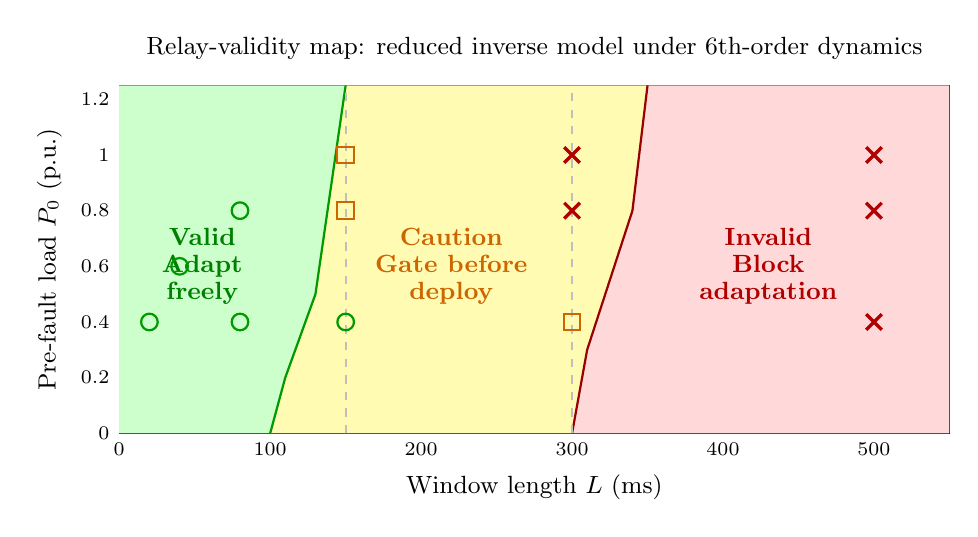
\begin{tikzpicture}
\begin{axis}[
  width=\columnwidth, height=6.0cm,
  xlabel={Window length $L$ (ms)},
  ylabel={Pre-fault load $P_0$ (p.u.)},
  xmin=0, xmax=550, ymin=0, ymax=1.25,
  xtick={0,100,200,300,400,500},
  ytick={0,0.2,0.4,0.6,0.8,1.0,1.2},
  ymajorgrids=true, xmajorgrids=true, grid style={gray!25},
  label style={font=\small},
  tick label style={font=\scriptsize},
  title={Relay-validity map: reduced inverse model under 6th-order dynamics},
  title style={font=\small},
  clip=false
]

%% --- Colored regions (fill first, then data) -----------------

% RED (Invalid): L > 300 ms (right region)
\addplot[fill=red!15, draw=none]
  coordinates {
    (300,0)(550,0)(550,1.25)(350,1.25)(340,0.8)(310,0.3)(300,0)
  } \closedcycle;

% YELLOW (Caution): between green boundary and red boundary
\addplot[fill=yellow!30, draw=none]
  coordinates {
    (100,0)(300,0)(310,0.3)(340,0.8)(350,1.25)
    (150,1.25)(130,0.5)(110,0.2)(100,0)
  } \closedcycle;

% GREEN (Valid): left region (L < ~100-150 ms)
\addplot[fill=green!20, draw=none]
  coordinates {
    (0,0)(100,0)(110,0.2)(130,0.5)(150,1.25)(0,1.25)(0,0)
  } \closedcycle;

%% --- Boundary lines ------------------------------------------
\draw[thick, green!60!black]
  plot coordinates {(100,0)(110,0.2)(130,0.5)(150,1.25)};
\draw[thick, red!60!black]
  plot coordinates {(300,0)(310,0.3)(340,0.8)(350,1.25)};

%% --- Region labels -------------------------------------------
\node[font=\small\bfseries, green!50!black, align=center]
     at (axis cs:55, 0.60)
     {Valid\\[-0.3ex]Adapt\\[-0.3ex]freely};
\node[font=\small\bfseries, orange!80!black, align=center]
     at (axis cs:220, 0.60)
     {Caution\\[-0.3ex]Gate before\\[-0.3ex]deploy};
\node[font=\small\bfseries, red!70!black, align=center]
     at (axis cs:430, 0.60)
     {Invalid\\[-0.3ex]Block\\[-0.3ex]adaptation};

%% --- Vertical guide lines ------------------------------------
\draw[thick, gray!50, dashed] (axis cs:150, 0) -- (axis cs:150, 1.25);
\draw[thick, gray!50, dashed] (axis cs:300, 0) -- (axis cs:300, 1.25);

%% --- Simulation data points ----------------------------------
% Valid cases: green circles
\addplot[only marks, mark=o, mark size=3pt,
         green!60!black, thick] coordinates {
  (20,0.4)(40,0.6)(80,0.8)(80,0.4)(150,0.4)
};

% Caution cases: orange squares
\addplot[only marks, mark=square, mark size=3pt,
         orange!80!black, thick] coordinates {
  (150,0.8)(150,1.0)(300,0.4)
};

% Invalid cases: red crosses
\addplot[only marks, mark=x, mark size=4pt,
         red!70!black, very thick] coordinates {
  (300,0.8)(300,1.0)(500,0.4)(500,0.8)(500,1.0)
};

\end{axis}
\end{tikzpicture}
